%Dies ist die Hauptseite des Dokumentes. Es werden u. a. alle Kapitel,
%Einstellung im Header eingebunden.
%Veränderungen müssen in folgenden Dateien vorgenommen werden:
      %- config.tex
      %- einzelne Kapitel (evtl. erweitern)

\input{common/layout.tex}          % Diese Datei enthält alle
                                          % Layouteinstellungen
\newcommand{\dokumentTitel}{Abnahmetestspezifikation}
% Definition von globalen Parametern, die derzeit auf der Titelseite und in der
% Kopfzeile verwendet werden. Der in <> gesetzte Text ist zu verändern.

\newcommand{\praktikumTitel}{<Titel des Praktikums>}
\newcommand{\projektTitel}{<Titel des Teilprojektes>}
\newcommand{\institut}{
	<Name des Instituts>\\
	<Name des Institutsleiters>\\
	<Straße und Hausnummer>\\
	<Postleitzahl und Ort>\\
}
\newcommand{\institutsLogo}{common/ISF_Logo.pdf}
\newcommand{\betreuer}{<Name>}


%------Beginn des Gesamtdokumentes----------------------------------------------
\begin{document}

%------Eingebundene Seiten, Verzeichnisse bzw. Kapitel--------------------------
\include{common/titelseite}                      % Titelseite


\tableofcontents                          % Inhaltsverzeichnis wird automatisch
                                          % generiert
%\listoffigures                            % ebenso das Abbildungsverzeichnis

%----Kapitel des Feinentwurfs, die mit Inhalt zu füllen sind--------------------
%!TEX root = ../Systementwurf.tex

\chapter{Einleitung}

\NewsGenie ist der persönliche Nachrichtensprecher. Immer auf dem neuesten
Stand und begierig darauf, die Fragen seiner Nutzer zu beantworten.
"`Was gibt es Neues in Russland?"', "`Wie hat Eintracht
Braunschweig gespielt?"', "`Wie alt ist Angela Merkel?"' - \NewsGenie
versteht seinen Benutzer ohne Tastatur, Suchmaske oder Bildschirm sondern in
völlig normaler Sprache.

Als Thin-Client-Server-Anwendung wird \NewsGenie so realisiert, dass der
Nutzer mittels eines kleinen und günstigen Clients auf das System
zugreifen und seine Anfragen stellen kann. Dabei hat er die Möglichkeit nach
Nachrichten aus einem Bereich, wie \glqq Technologie\grqq\, einem bestimmten aktuellen Thema, wie der Ukraine, sowie nach Fakten,
z.B. dem Alter einer Person des öffentlichen Lebens, zu suchen.

Um dies zu realisieren, wird dem Server eine maßgebliche Rolle zuteil. Dieser verarbeitet die Anfragen der verschiedenen Clients, 
erfasst parallel die einzelnen Nachrichtenartikel von den in der Datenbank
hinterlegten Newsseiten und stellt den Nutzern ein Webinterface zur Verfügung.

Der Server basiert auf einer 3-Schichten-Architektur aus
Benutzerschnittstelle, System- und Persistenzschicht und wird in Java
entwickelt.
Die Benutzerschnittstelle besteht auf der Serverseite aus dem Webinterface, das mit Hilfe des Play-Frameworks\footnote{Mit dem quelloffenen Play-Framework kann man einfach ressourcenschonende Web-Applikationen in Java und Scala entwickeln. \url{http://www.playframework.com/}} realisiert wird.
Die Systemschicht stellt die Kernfunktionalität des Servers bereit, das Annehmen von Anfragen, deren Verarbeitung mit Hilfe von "`Natural Language Processing"'\footnote{Stanford CorNLP, eine Sammlung von Sprachanalysetools. Verwendet werden der Part-of-Speech tagger (POS) und der Named Entity Recognizer (NER), \url{http://nlp.stanford.edu/software/corenlp.shtml}} und außerdem den Crawler, welcher regelmäßig die hinterlegten Newsseiten nach neuen Artikeln durchsucht und in der Persistenzschicht, einer Datenbank realisiert mit einem Virtuoso\footnote{OpenLink Virtuoso ist ein quelloffenes Datenbanksystem, das die Funktionalität vieler verschiedener Datenbankparadigmen kombiniert. Wird hier als Triple-Store verwendet. \url{http://virtuoso.openlinksw.com/dataspace/doc/dav/wiki/Main/}} Triple-Store, speichert. 
Die Datenbank ist außerdem mit einem Lucene-Index versehen.

%
%Die Benutzerschnittstelle besteht auf der Serverseite aus dem Webinterface.
%In diesem kann sich der Benutzer registrieren und nach einem Login Textanfragen stellen
%und seine Nachrichtenquellen verwalten. 
%Weiterhin besteht die Möglichkeit, sein Passwort zu ändern oder wiederherzustellen und 
%seinen Account zu löschen. Administratoren können außerdem in die Sicht von anderen
%Benutzern wechseln und diese löschen. Das Webinterface wird mit Hilfe des Play-Frameworks realisiert.
%
%Die Systemschicht stellt die Kernfunkionalitäten des Servers bereit. Der
%Management-Handler nimmt alle Anfragen von Clients und aus dem Webinterface entgegen 
%und koordinert die weiteren Schritte. Handelt es sich dabei ausschließlich um eine Anfrage nach Daten,
%wie zum Beispiel bei einem Login-Versuch, wo geprüft werden muss, ob ein Nutzername registriert ist, 
%werden diese Informationen aus der Datenbank gesucht und die Anfrage so beantwortet. Handelt es sich 
%jedoch um eine Anfrage nach Neuigkeiten, besteht diese aus natürlicher Sprache und muss zunächst interpretiert werden.
% Hierzu wird die eingegangene Anfrage
% durch "`Natural Language Processing"' analysiert und durch
%unser eigenes Analysetool geschickt, welches die enthaltenen Wörter in einen Kontext setzt.
%Anschließend werden die am Besten zur Anfrage passenden Artikel aus der Datenbank gesucht und das
% Ergebnis wieder in einen natürlichen Satz umgewandelt.
%Außerdem beinhaltet die Systemschicht den Crawler, welcher die in der Datenbank
%hinterlegten Newsseiten regelmäßig nach neuen Artikeln durchsucht.
%
%Die Persistenzschicht beinhaltet einen Virtuoso-Triplestore, der als Datenbank dient, 
%sowie einen Lucene-Index zur effizienten Volltextsuche. 
%In Virtuoso werden die Daten der Benutzer sowie Feeds und deren beinhaltete Artikel gespeichert.

Alle Schichten kommunizieren mit Hilfe des Akka-Frameworks\footnote{Akka ist ein Framework zur Entwicklung fehlertoleranter, verteilter Java- und Scala Anwendungen, basierend auf dem Aktoren-Modell. \url{http://akka.io/}}, welches einen sicheren,
asynchronen Datenaustausch ermöglicht.

Aus der genannten Aufteilung resultieren die in Abb. \ref{komponenten}
dargestellten Komponenten.

In den nachfolgenden Abschnitten wird die Implementierung \NewsGenie vorgestellt. Zunächst die Komponentenaufteilung, gefolgt von Implementierungsdetails wie den einzelnen Funktionen und dem Datenmodell.

\begin{figure}[h]
\centering
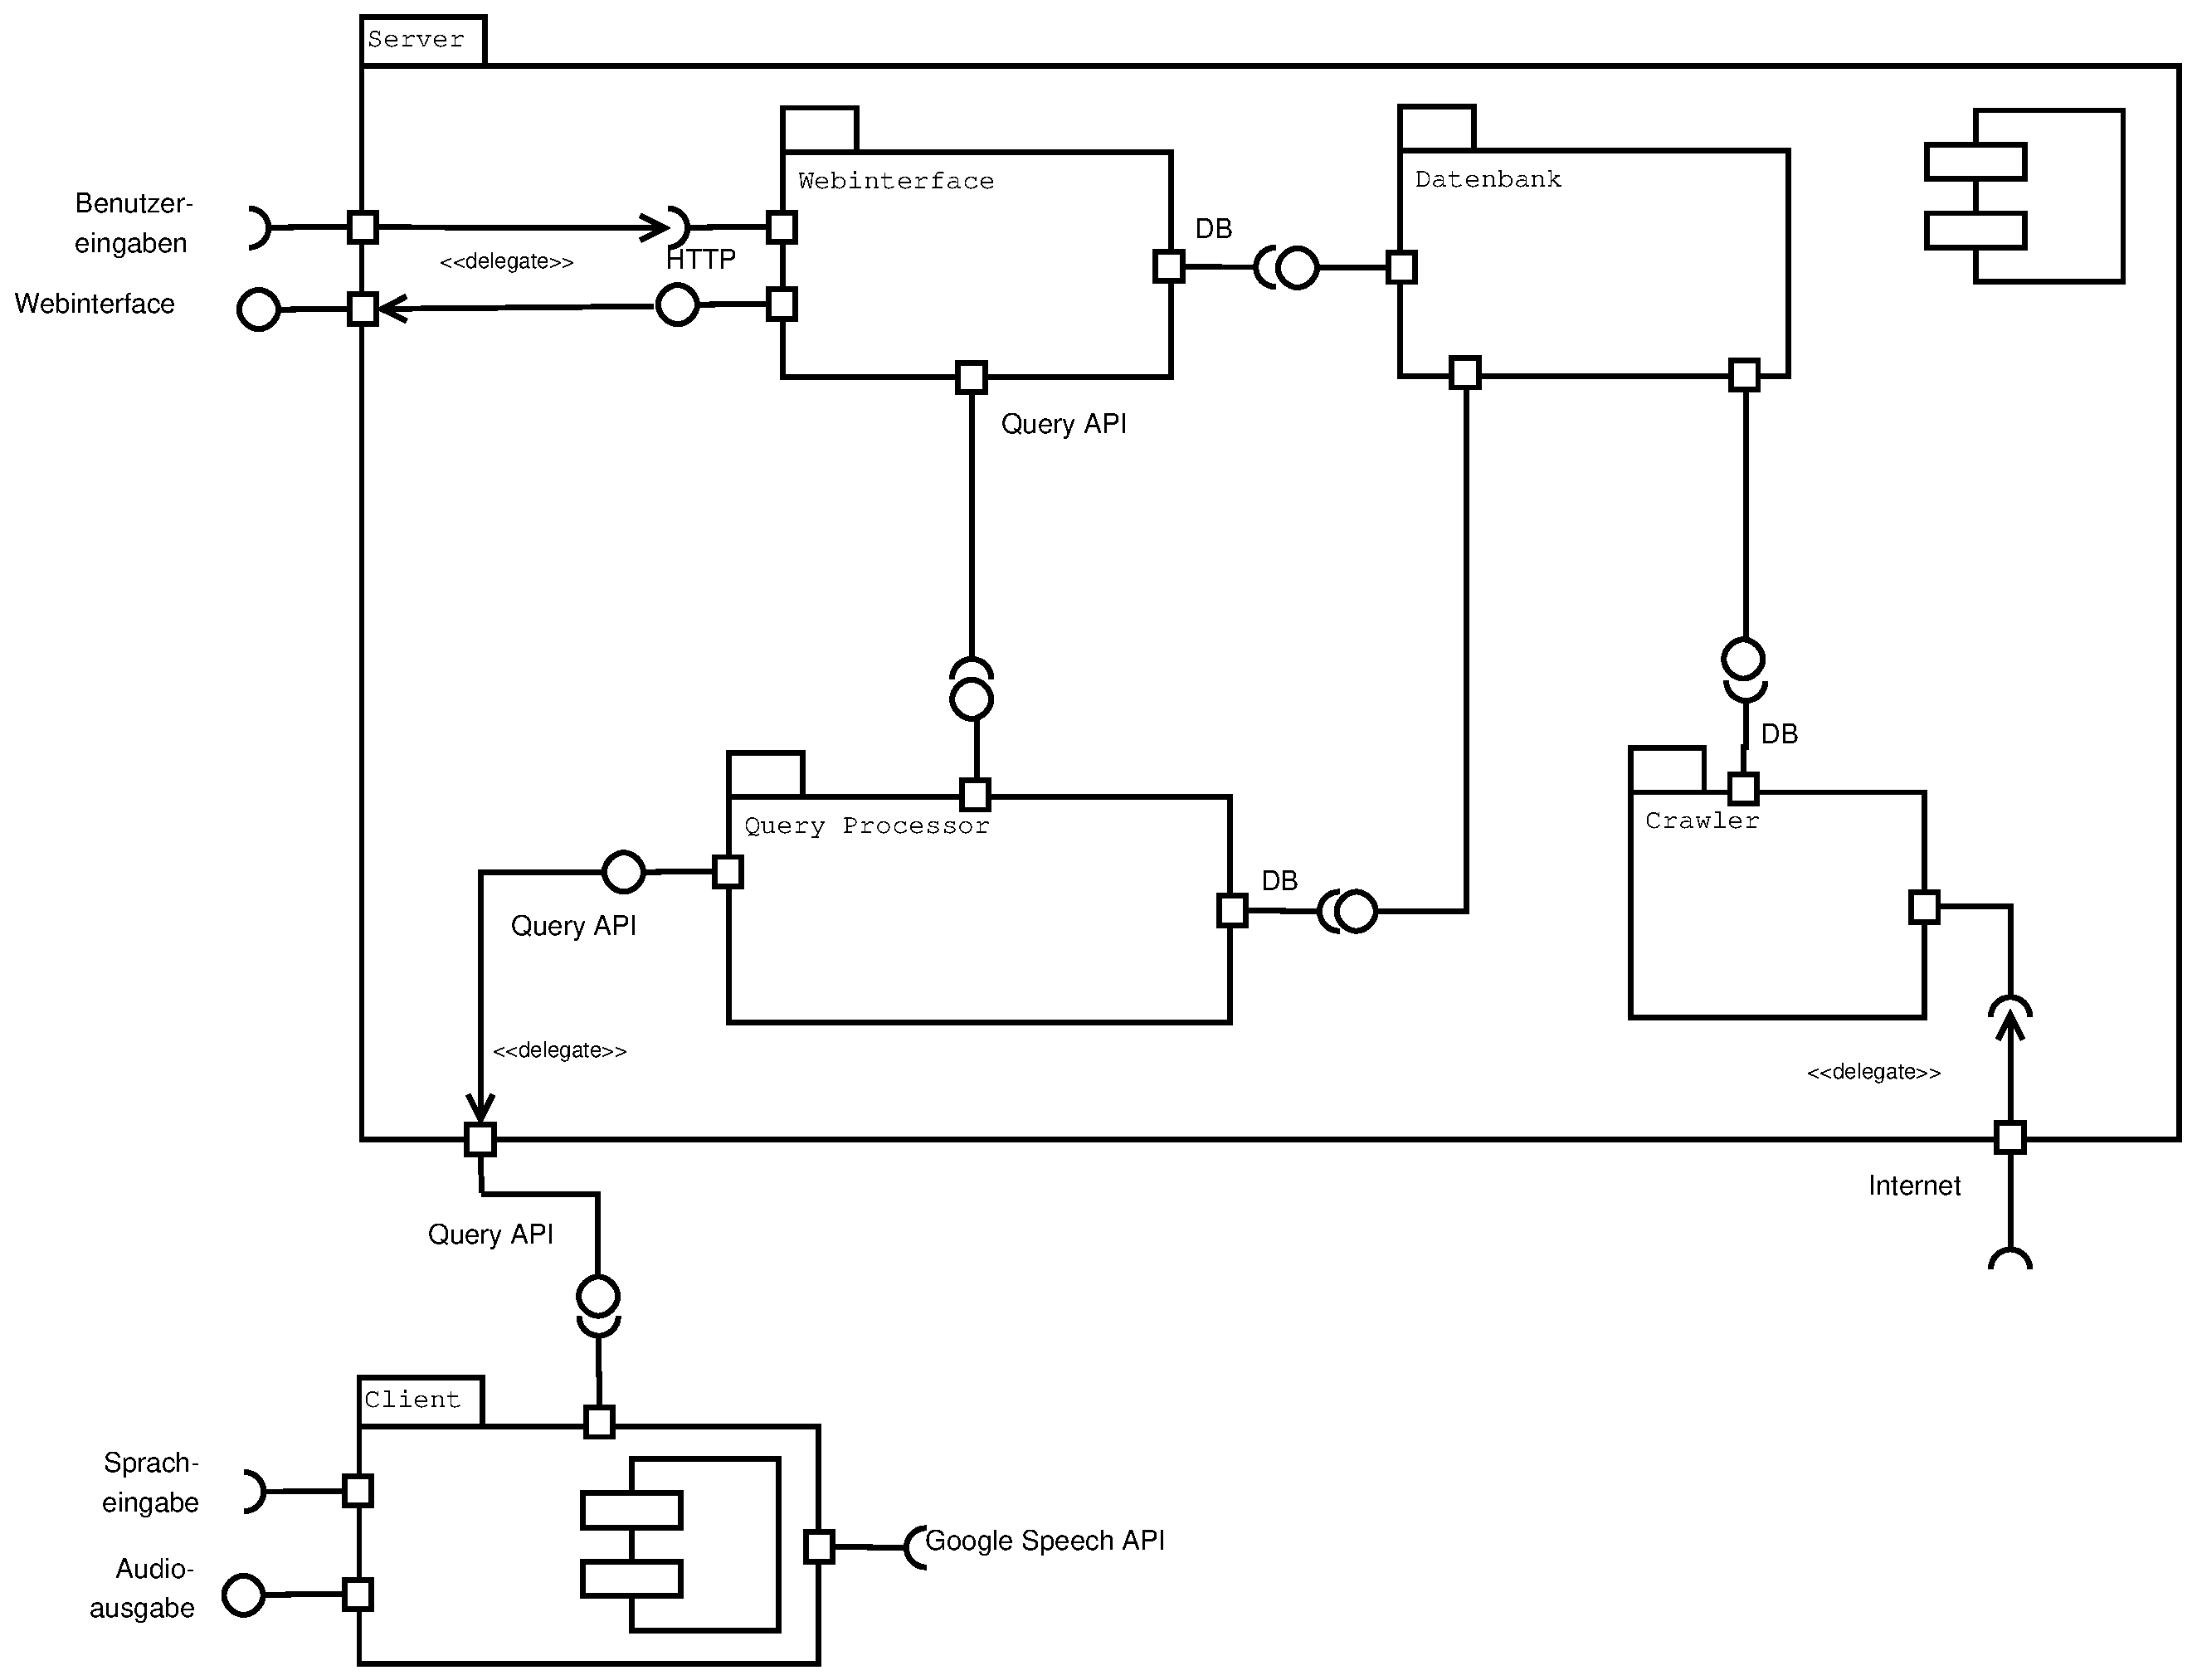
\includegraphics[width=1\textwidth]{Systementwurf/05_implementierungsentwurf/komponenten}
\caption{Komponentendiagramm, \textit{Komponentenaufteilung von \NewsGenie}
\label{komponenten}}
\end{figure}

\FloatBarrier
\section{Projektdetails}

Um wichtige Aspekte von \NewsGenie genauer zu erläutern, werden in diesem
Kapitel verschiedene Funktionen der Anwendung aufgeführt und beschrieben. In den folgenden
Unterkapiteln werden das Registrieren, die Anmeldung am Webinterface, das Hinzufügen von Feeds
 und die Interaktion zwischen Benutzer und Client genauer erklärt.

\subsection{Registrieren und Anmelden}

Die folgenden Aktivitätsdiagramme~\ref{1.2}~und~\ref{1.3} beschreiben den Workflow bei der Registrierung
 und Anmeldung eines Nutzers. Will
sich ein Nutzer registrieren um \NewsGenie zu nutzen, so muss er im Webinterface
den entsprechenden Registrierungs-Button anklicken. Dadurch wird ihm vom System
die Seite angezeigt, auf der er seinen gewüschten Benutzernamen und sein selbst
gewähltes Passwort sowie seine E-Mail-Adresse in Textfelder eintragen kann.
Nachdem der Nutzer seine Eingaben bestätigt hat, legt das System
seine Daten in der Datenbank ab, sofern sie nicht schon vergeben waren.
 Nun kann der Nutzer sich am Client und im
Webinterface anmelden. Über den Client kann er anschließend Anfragen stellen
oder über das Webinterface seine Einstellungen verwalten bzw. eine Textanfrage
stellen.

\begin{figure}[h]
\centering
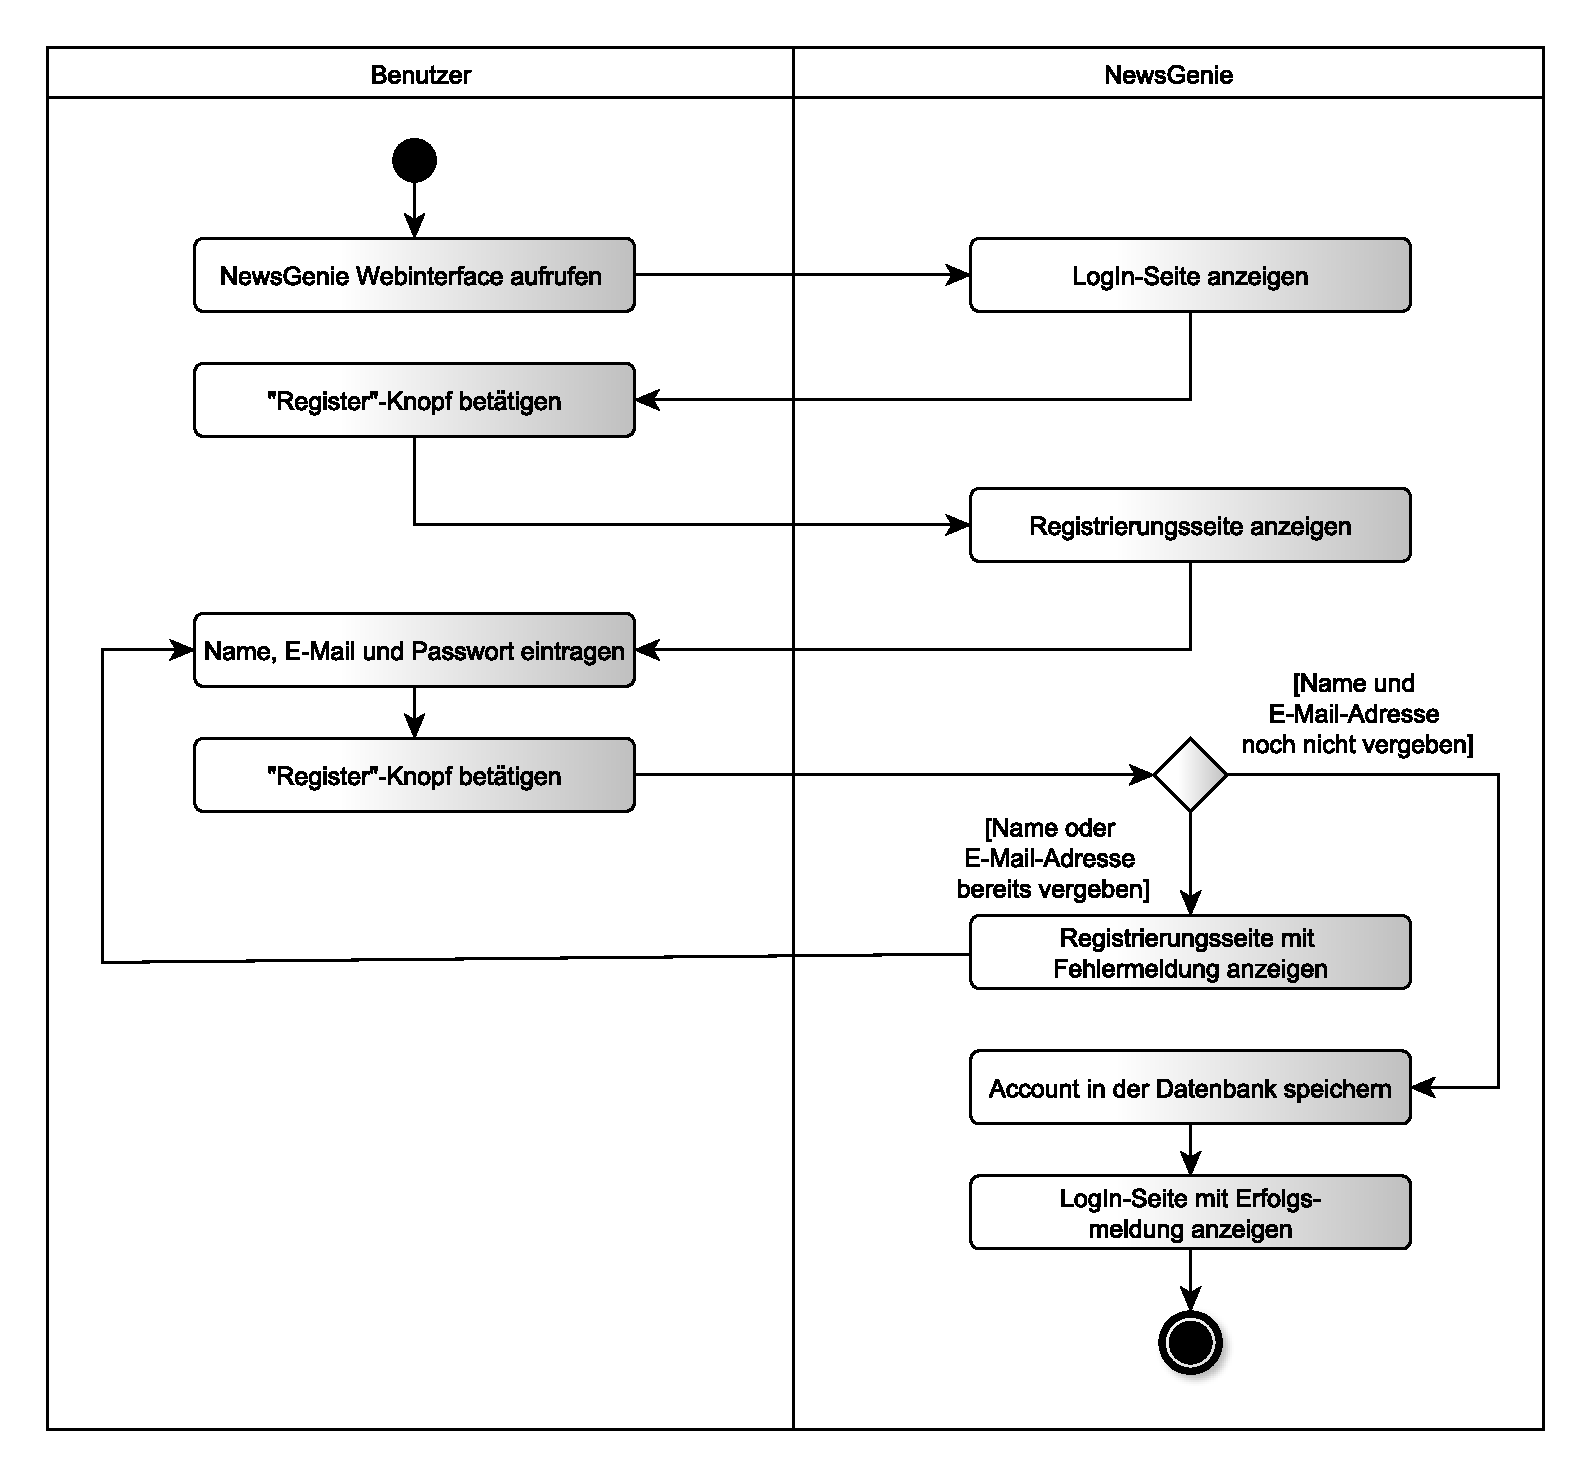
\includegraphics[width=1\textwidth]{Systementwurf/01_einleitung/register.eps}
\caption{Aktivitätsdiagramm, \textit{Registrierung bei \NewsGenie}
\label{1.2}}
\end{figure}

\begin{figure}[h]
\centering
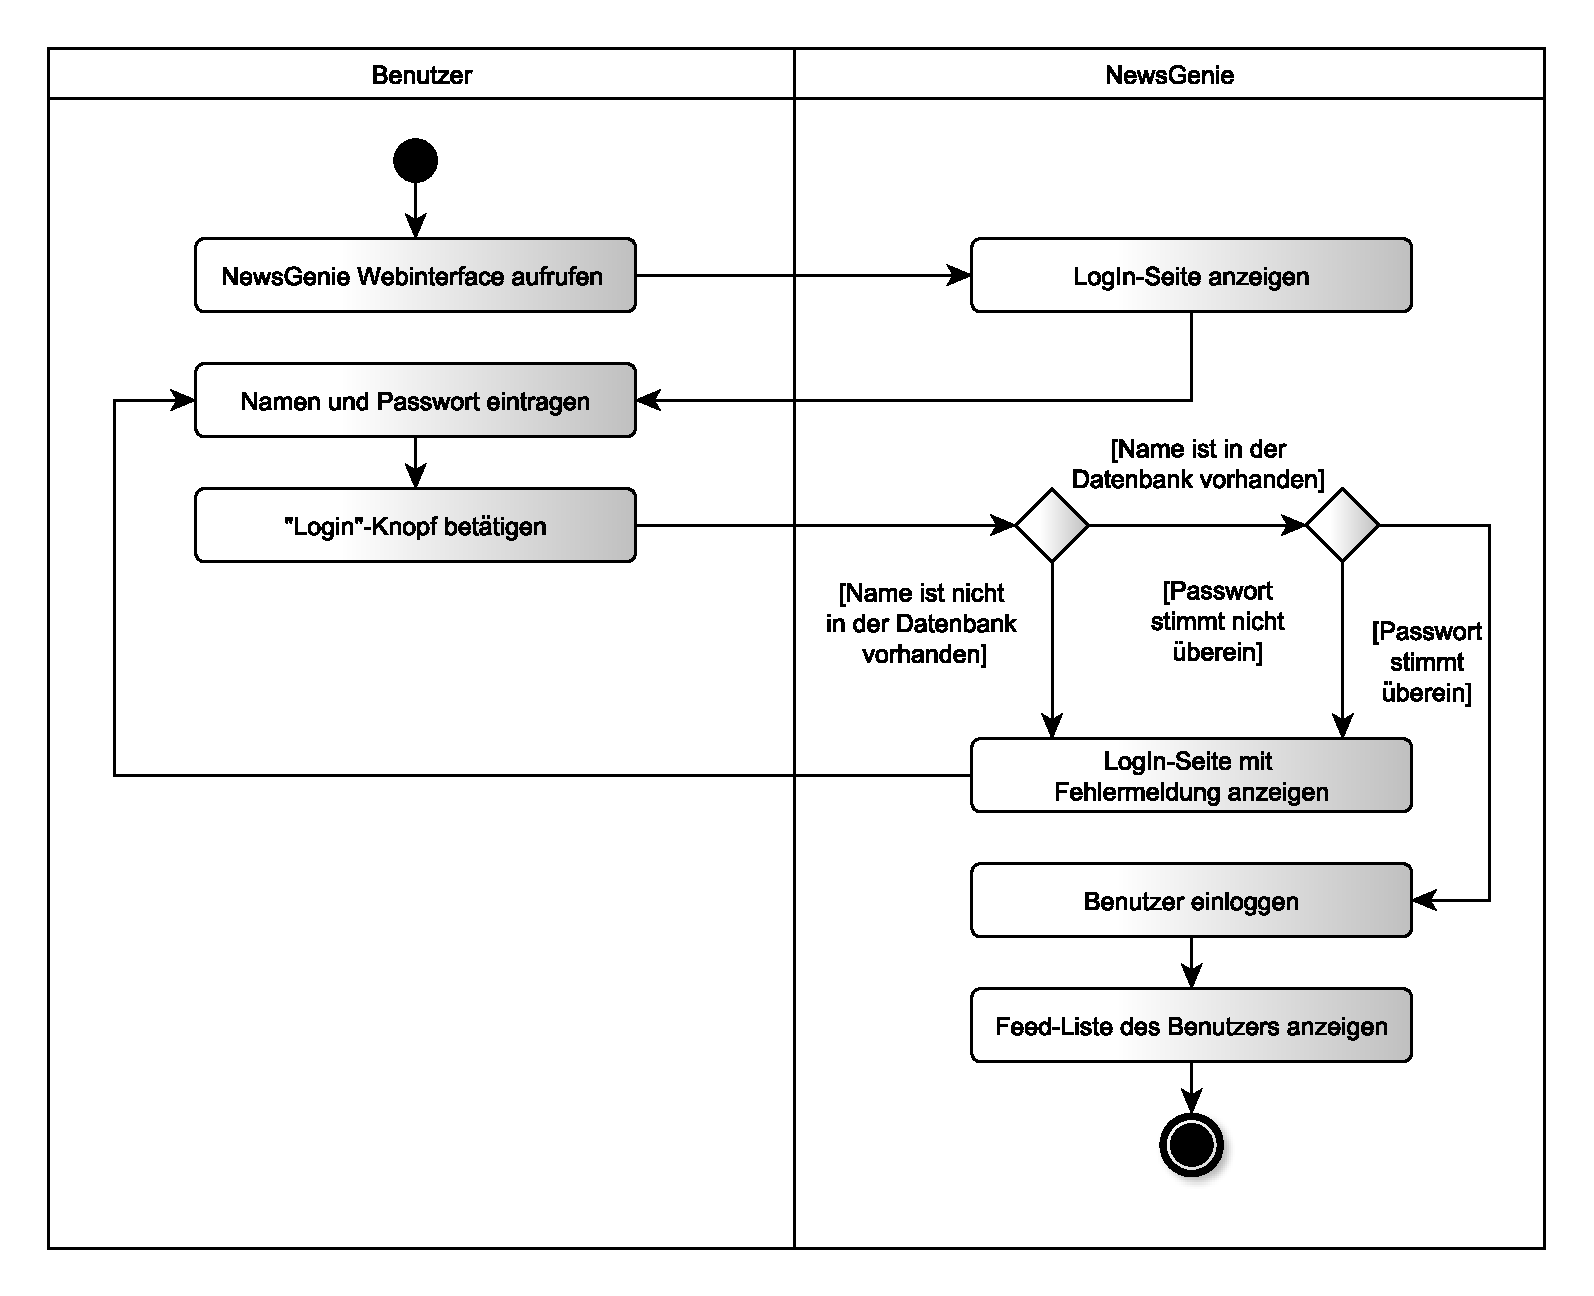
\includegraphics[width=1\textwidth]{Systementwurf/01_einleitung/weblogin.eps}
\caption{Aktivitätsdiagramm, \textit{Anmeldung am Webinterface}
\label{1.3}}
\end{figure}

\subsection{Feeds hinzufügen}

Sobald ein Benutzer sich am Webinterface eingeloggt hat, besteht für ihn die Möglichkeit, 
seine Feeds zu verwalten. Im nachfolgenden Aktivitätsdiagramm~\ref{1.4} wird dargestellt,
wie ein Benutzer neue Feeds abonnieren kann. Es reicht dazu aus, die URL des hinzuzufügenden 
Feeds in das dazu vorgesehene Textfeld einzugeben und die Eingabe per Knopfdruck zu bestätigen.
Das System prüft nun ob unter der angegebenen URL tatsächlich ein Feed zu finden ist und gibt sonst
eine Fehlermeldung aus. Falls der Feed existiert, wird er in der Datenbank gespeichert, falls dies noch nicht der Fall ist, und der Benutzer wird ihm als Abonnent zugeordnet.

\begin{figure}[h]
\centering
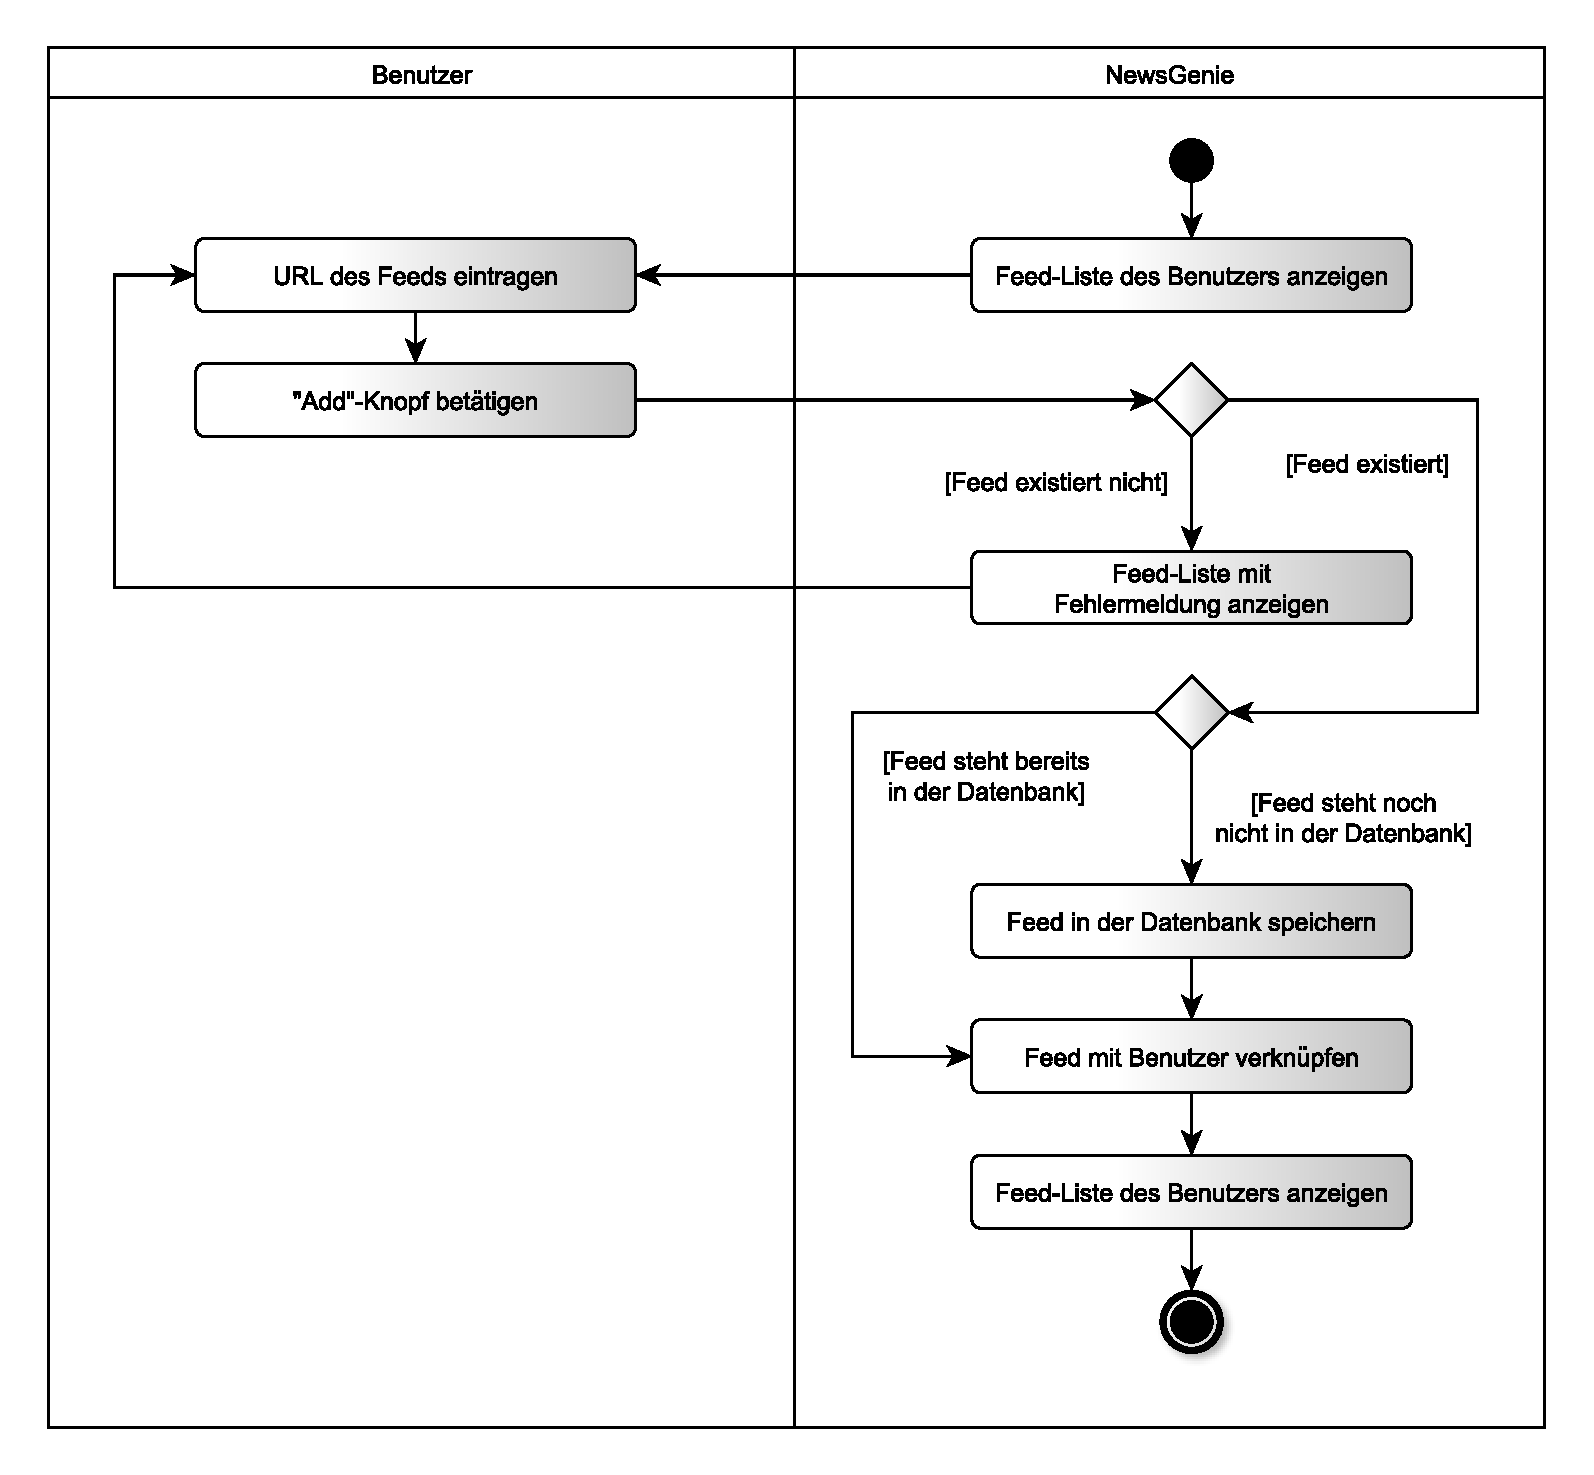
\includegraphics[width=1\textwidth]{Systementwurf/01_einleitung/addfeed.eps}
\caption{Aktivitätsdiagramm, \textit{Hinzufügen von Feeds}
\label{1.4}}
\end{figure}

\pagebreak[3]

\subsection{Interaktion zwischen Benutzer und Client}

Die verbale Kommunikation zwischen Benutzer und Client ist der Kern von \NewsGenie 
und zu komplex um sie komplett in einem Aktivitätsdiagramm darzustellen.
Folgende Funktionen sollen bereit gestellt werden:
\begin{itemize}
\item Login und Logout
\item Anfragen nach Neuigkeiten allgemein
\item Anfragen nach Neuigkeiten zu einem Thema
\item Erweiterung von Anfragen
\item Eingrenzung von Anfragen
\item Anfragen nach Fakten
\end{itemize}
Hierbei soll \NewsGenie möglichst selbstständig erkennen, was der Benutzer möchte und worauf sich
Anfragen beziehen. Insbesondere sol der Nutzer in der Lage sein, \NewsGenie zu jedem Zeitpunkt zu unterbrechen.

Ein relativ einfacher beispielhafter Workflow ist hierzu in Aktivitätsdiagramm~\ref{1.5} abgebildet.
Dieser Ablauf ist dabei nur einer von vielen. Durch die Kommunikation mittels Sprache hat der Nutzer zu jeder Zeit
viele verschiedene Möglichkeiten den Ablauf zu verändern.
Zusätzlich kann es immer passieren, dass Eingaben nicht verstanden werden und \NewsGenie nachfragen muss.
Die Verarbeitung einer Anfrage wird in Aktivitätsdiagramm~\ref{1.6} dargestellt.

\begin{figure}[h]
\centering
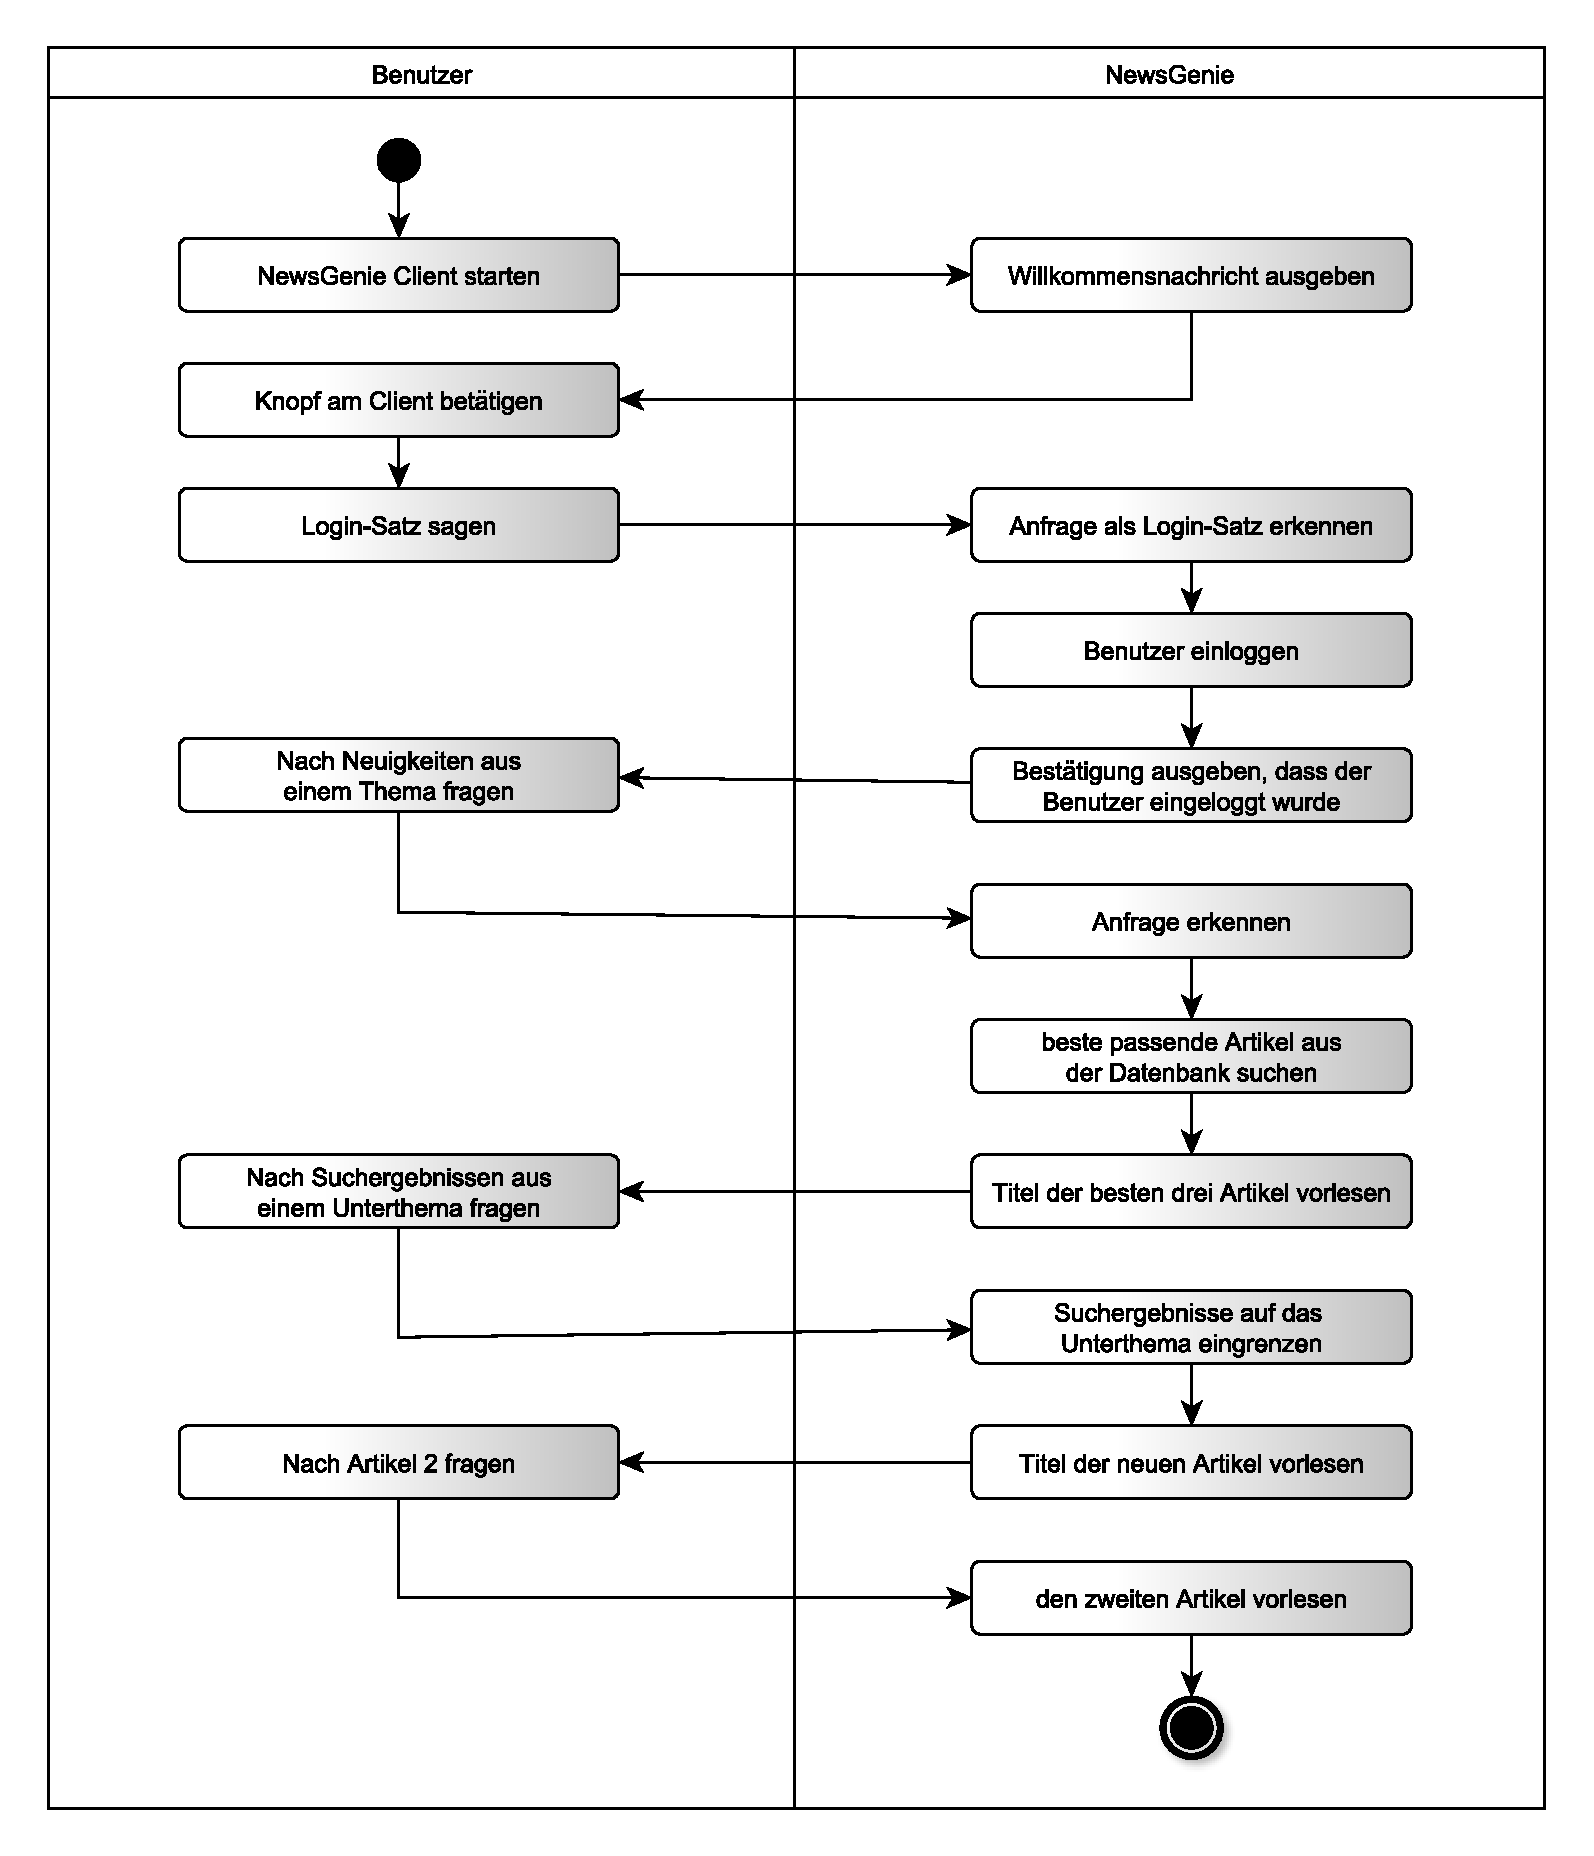
\includegraphics[width=1\textwidth]{Systementwurf/01_einleitung/conversation.eps}
\caption{Aktivitätsdiagramm, \textit{Beispielhafte Kommunikation mit dem Client}
\label{1.5}}
\end{figure}

\begin{figure}[h]
\centering
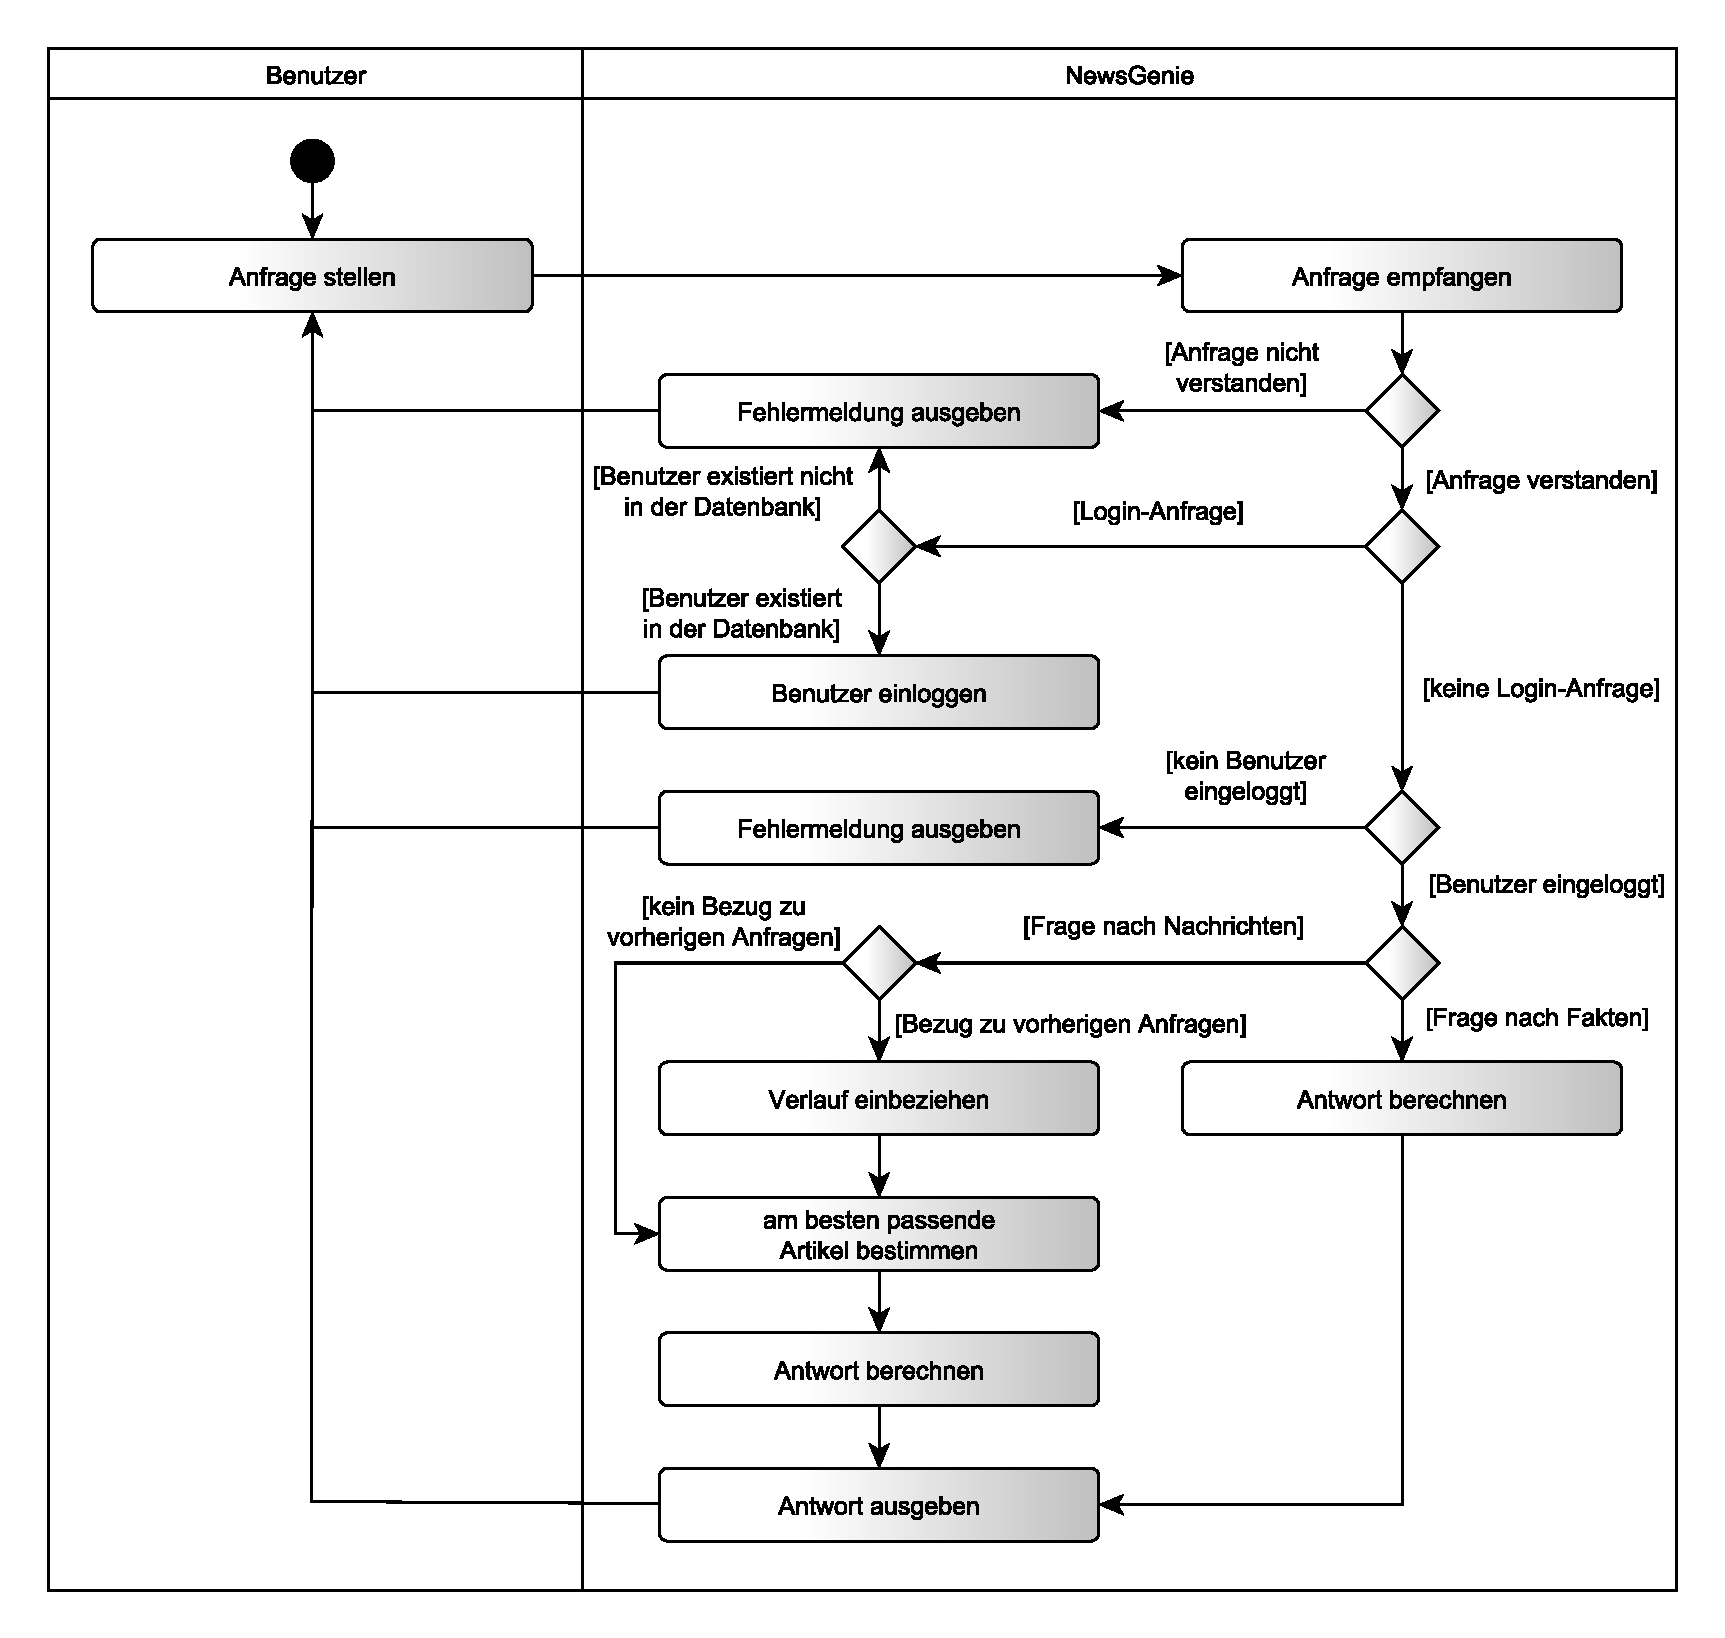
\includegraphics[width=1\textwidth]{Systementwurf/01_einleitung/request.eps}
\caption{Aktivitätsdiagramm, \textit{Verarbeitung einer Anfrage}
\label{1.6}}
\end{figure}

\iffalse
Die zwei Aktivitätsdiagramme in Abbildung \todo[inline]{Referenz} und
\todo[inline]{Referenz} zeigen den Workflow von \NewsGenies Hauptaufgabe, dem
Stellen einer Anfrage an das System.
Hierbei wird vorausgesetzt, dass sich der Nutzer bereits registriert und
entweder (je nach Anfragetyp) am Client oder im Webinterface angemeldet hat.
Will der Nutzer nun eine Anfrage am Client an \NewsGenie stellen, so spricht er
seine Frage. Die Anfrage durchläuft das System und eine Antwort wird
anschließend durch den Client ausgegeben. Dabei hängt die Antwort von dem
Ergebnis der Speech-To-Text- und der eigenen Analyse ab. Kann \NewsGenie zum
Beispiel keine Eingabe bzw. Frage feststellen, so gibt er eine entsprechende
Antwort mit Aufforderung zur Wiederholung der Eingabe auf.
Will der Nutzer stattdessen eine Anfrage im Webinterface an \NewsGenie stellen,
so tippt er seine Frage in das entsprechende Textfeld seine Frage. Nach dem
Klicken auf den "`Ask"'-Button, durchläuft die Anfrage genauso wie beim Client
das System und eine Antwort wird anschließend durch den Client ausgegeben.
Allerdings ist die Wahrscheinlichtkeit einer erfolgreichen Frage hier höher, da
Speech-To-Text hier nicht gebraucht und so die Fehlerwahrscheinlichkeit
minimiert wird.


\todo[inline]{Diagramm 1 - Client}
\todo[inline]{Diagramm 2 - Webinterface}
\fi
%!TEX root = ../Testspezifikation.tex

\chapter{Testplan}

Im Folgenden wird der Testplan für SQL-Alchemist beschrieben. Dabei wird sowohl auf die zu testenden Komponenten als auch die bereits im Pflichtenheft beschriebenen Funktionen und Merkmale eingegangen. Außerdem wird noch das genaue Vorgehen bei der Durchführung der Tests aufgezeigt.

\section{Zu testende Komponenten}

Die Sofware besteht grundsätzlich aus zwei Komponenten: Front-End und Back-End.\\
Da diese jedoch auf verschiedene Weise an verschiedenen Teilen der Software beteiligt sind, sind folgend die verschiedenen Kernpunkte aufgelistet, die zur Bewertung der Funktionstüchtigkeit getestet werden müssen:

\begin{itemize}
\item \textbf{SQL Modul: }Das SQL Modul ist der Kern der Software. Der Zweck des Programms, nämlich der Unterstützung beim Erlernen der Datenbankanfragesprache SQL, wird hierüber realisiert. Daher muss besonders die korrekte Anzeige der Aufgaben und die automatische Bewertung getestet werden. Weiterhin soll eine simple Bedienbarkeit gewährleistet werden.
\item \textbf{Minispiel: }Das Minispiel stellt die zweite zentrale Komponente des Projektes dar und muss daher auch ausgiebig getestet werden. In diesem Fall liegt das Hauptaugenmerk auf der Spielbarkeit der einzelnen Level und die Einhaltung des Schwierigkeitsgrades.
\item \textbf{GUI: }Die grafische Oberfläche bildet die Schnittstelle zwischen Benutzer und Applikation. Daher muss hier geprüft werden, ob die Menüs auf allen Endgeräten korrekt angezeigt werden und intuitiv bedienbar sind.
\item \textbf{Datenbank: }Die Datenbank ist für die Speicherung aller Daten notwendig, die für die Erstellung der SQL-Abfragen benötigt werden. Demnach muss die Konsistenz und die Sicherung der Daten geprüft werden um einen einfachen Zugriff sicherzustellen.
\item \textbf{Benutzerverwaltung: }Die Benutzerverwaltung sorgt für die Speicherung der Spieleraccounts. In diesem Fall muss insbesondere die korrekte Rechtevergabe getestet werden.
\item \textbf{Ranglisten/Spielerprofile: }Die Profile halten den Fortschritt der Spieler fest, während die Ranglisten es ermöglichen, dass sich die Nutzer untereinander messen können. Daher ist es wichtig, dass alle zu erfassenden Daten in gewünschter Weise abgespeichert und angezeigt werden.
\item \textbf{Administrationstool: }Das Administrationstool ist das Werkzeug, welches benötigt wird damit die Dozenten und ihre Mitarbeiter das Spiel vorlesungsunterstützend einsetzen können. Die gesamte Hausaufgabenverwaltung läuft über dieses Tool. Demnach muss an dieser Stelle getestet werden, ob die Erstellung neuer Eingaben intuitiv und schnell machbar ist.
\end{itemize}

\section{Zu testende Funktionen/Merkmale}

Um die oben genannten Kernpunkte der Software effizient zu testen bietet sich an, die Produktfunktionen zu Hilfe zu nehmen. Zu diesem Zweck sind diese hier noch einmal aufgefürt und kurz umschrieben. 

\begin{itemize}
\item \textbf{$\langle$F10$\rangle$ Nutzer registrieren: }Neue Benutzer lassen sich durch Angabe von E-Mail/y-Adresse, sowie Passwort registrieren. Dabei wird auf die Vollständigkeit der Angaben geachtet und Studenten werden automatisch anhand der Eingaben erkannt.
\item \textbf{$\langle$F20$\rangle$ Nutzer anmelden: }Die Nutzer-Authentifizierung erkennt, ob es sich um einen registrierten Nutzer handelt und gewährt diesem Zugang.
\item \textbf{$\langle$F30$\rangle$ Nutzer abmelden: }Der Nutzer wird ordnungsgemäß abgemeldet und kann, ohne erneute Anmeldung, nicht mehr auf das Spiel zugreifen.
\item \textbf{$\langle$F40$\rangle$ Profil einsehen: }Das Profil wird auf allen Endgeräten korrekt und gut lesbar dargestellt. Alle angezeigten Daten sind richtig und aktuell.
\item \textbf{$\langle$F60$\rangle$ Passwort ändern: }Das Passwort wird geändert, der Passworthash in der Datenbank aktualisiert sich dabei. Anschließend muss sich der Nutzer mit dem neuen Passwort anmelden können, das alte Passwort ist nicht mehr gültig.
\item \textbf{$\langle$F70$\rangle$ Avatar ändern: }Die Spielfigur im Minispiel und das Icon das Nutzers werden geändert und korrekt dargestellt.
\item \textbf{$\langle$F90$\rangle$ Audioeinstellungen bearbeiten: }Soundeffekte und Musik können unabhängig voneinander ein- und ausgeschaltet werden. Die Einstellung wird korrekt in der Datenbank gespeichert und bei der nächsten Anmeldung korrekt geladen.
\item \textbf{$\langle$F100$\rangle$ Spielstand zurücksetzen: }Der Spielstand wird korrekt zurückgesetzt. Das Tutorial bleibt deaktiviert.
\item \textbf{$\langle$F110$\rangle$ Tutorial spielen: }Das Tutorial ist standardmäßig bei einem neuen Nutzer aktiviert, bis dieser das Tutorial erfolgreich beendet hat. Dann wird das Tutorial automatisch deaktiviert,  bis es im \glqq Settings\grqq-Menü erneut aktiviert wird.
\item \textbf{$\langle$F120$\rangle$ Story spielen: }Der Ablauf der Handlung ist korrekt und das Zusammenspiel von Minispiel und SQL-Modul funktioniert wie geplant.
\item \textbf{$\langle$F130$\rangle$ SQL-Trainer spielen: }Die Aufgaben wiederholen sich im Trivia-Modus nicht zu häufig. Im Story-Modus werden zu jedem Zeitpunkt die aktuellen Aufgaben gestellt. Zudem darf es nicht zu Fehlern kommen, die die Bearbeitung einschränken. Die Rückmeldung auf die Antwort der Nutzer ist korrekt. 
\item \textbf{$\langle$F140$\rangle$ Minispiel spielen: }Durch den zufälligen Aufruf der Level kommt es nicht zu Wiederholungen. Die Figur reagiert sofort auf Eingaben und das Spiel ist auf allen Endgeräten spielbar.
\item \textbf{$\langle$F150$\rangle$ Hausaufgaben bearbeiten: }Es werden die geforderten Aufgabenpakete geladen und die Bewertung funktioniert wie erwünscht. Bei der Bearbeitung darf es nicht zu Fehlern kommen, die den Betrieb einschränken.
\item \textbf{$\langle$F160$\rangle$ Ranglisten einsehen: }Die Ranglisten stellen alle geforderten Daten aktuell und richtig dar.
\item \textbf{$\langle$F170$\rangle$ Spieler suchen: }Spieler sollen anhand ihres Benutzernamens gesucht und korrekt angezeigt werden.
\item \textbf{$\langle$F180$\rangle$ Hausaufgabenergebnisse einsehen: }Die in den Hausaufgaben erzielten Ergebnisse werden ordnungsgemäß abgespeichert und für jeden Nutzer sind nur die eigenen Ergebnisse einsehbar.
\item \textbf{$\langle$F200$\rangle$ Benutzer Adminrechte geben: }Die Option kann nur von einem Admin genutzt werden und ernennt nur den richtigen Benutzer zum Admin.
\item \textbf{$\langle$F210$\rangle$ Trivia-Aufgabe erstellen: }Nur berechtigte Nutzer haben Zugriff auf diese Funktion und die Aufgaben werden korrekt und vollständig in die Datenbank eingepflegt.
\item \textbf{$\langle$F220$\rangle$ Benutzeraufgaben bewerten: }Die Bewertung kann nur von Admins oder beförderten Nutzern vorgenommen werden und wird korrekt mit den bereits vorhandenen Bewertungen verrechnet.
\item \textbf{$\langle$F230$\rangle$ Hausaufgaben erstellen: }Hausaufgaben können nur von Admins erstellt und nur von Studenten bearbeitet werden. Die Hausaufgaben sind nur innerhalb des angegebenen Bearbeitungszeitraums freigeschaltet.
\item \textbf{$\langle$Q10$\rangle$ Benutzerfreundlichkeit: }Alle Funktionen sind für den Nutzer verständlich und können über möglichst kurze Wege durch das Menü erreicht werden.
\item \textbf{$\langle$Q20$\rangle$ Zuverlässigkeit: }Das Spiel stürzt nicht ab und die Bearbeitung der Hausaufgaben ist technisch jederzeit möglich.
\item \textbf{$\langle$Q30$\rangle$ Korrektheit: }Die Auswertung der Benutzereingaben ist korrekt.
\item \textbf{$\langle$Q40$\rangle$ Plattformunabhängigkeit: }Das Spiel ist plattformunabhängig nutzbar.
\end{itemize}
 

\section{Nicht zu testende Funktionen}

Bei allen verwendeten Frameworks und Funktionen von Dritten werden ausreichende Testläufe vorausgesetzt. Daher werden keine weiteren Tests für die folgende Software vorgenommen:
\begin{itemize}
\item MelonJS (Framework)
\item play (Framework)
\item jQuery (Framework)
\item AngularJS (Framework)
\item Bootstrap (Framework)
\item automatische Generierung von Schemata und Statements (Teamprojekt)
\end{itemize}

\section{Vorgehen}

\textbf{a) Abnahme- und Funktionstests:} \\
Für den Abnahmetest ist folgendes Vorgehen geplant: Damit der Kunde einen guten Gesamtüberblick über alle Funktionalitäten erhält, sollen alle Anwendungsfälle aus der Anforderungsspezifikation in einer Reihenfolge getestet werden, in der auch spätere Nutzer die Applikation nutzen könnten. 
Dazu wird sich der Kunde zuerst einen neuen Account erstellen, dem dann der Administrator-Status zugewiesen wird. Mit diesem Account kann er zunächst, unabhängig vom eigentlichen Programm, die verschiedenen Funktionen des Administrationstools testen. Danach wird er sich für die eigentliche Applikation anmelden um die unterschiedlichen zur Verfügung stehenden Funktionen auszuprobieren und auch die verschiedenen Spielmodi anzuspielen. Zuletzt wird der Kunde dann noch die Abmeldung durchführen.
Während dieses Testlaufs kann sich der Kunde dann auch gleich ein Bild davon machen, inwieweit die im Pflichtenheft festgelegten Qualitätsstandards eingehalten wurden.\\

\newpage
 \textbf{b) Integrationstest:} \\
 Im Integrationstest wird für diese Software die Komunikation der beiden Komponenten getestet.\\
 Da die Komponenten über verschiedene Schnittstellen miteinander kommunizieren, werden für den Integrationstest die Funktionen nochmal genauer beleuchtet, die die jeweilige Schnittstelle benutzen. Dabei werden die Funktionen manuell mehrfach ausgeführt um die stabilität der Daten zu gewährleisten. Desweiteren werden die angezeigten Daten dabei mit den Daten in der Datenbank verglichen.  \\ 
 
 \textbf{c) Unittest:} \\
 Bei den Unit-Tests werden die einzelnen Komponenten für sich selbst überprüft. 
 Dies geschieht für das Back-End schon während der Programmierung. Da das Back-End zum Großteil eine Java-Basierte Anwendung ist wird beim Testen Gebrauch von JUnit gemacht, es wird also für jede erstellte Klasse direkt ein Test erstellt.
 Da das Front-End eine Javascript-basierte Anwendung ist und sich Unittests dafür nur etwas zeitaufwendiger umsetzen lassen wurde von diesen, in Absprache mit dem Protokoll-abnehmenden Institut, abgesehen.

\section{Testumgebung}
 Back-End Funktionen werden mit der JUnit getestet. Diese ist in das benutzte play!-Framework integriert.
Tests für Front-End Funktionen werden manuell durchgeführt.
 





%Der Testplan ist das zentrale Dokument der Qualitätssicherung und wird daher
%frühzeitig erstellt. Hier wird Umfang und Vorgehensweise der Qualitätssicherung
%beschrieben. Außerdem werden Testgegenstände und deren zu testenden
%Eigenschaften bzw. Funktionen identifiziert. Ferner werden die
%durchzuführenden Maßnahmen und die dafür verantwortlichen Personen definiert.
%Falls erforderlich sollte hier auch auf allgemeine Risiken eingegangen werden.


%\textbf{Dieses Kapitel kann aus der Abnahmetestspezifikation übernommen werden, 
%sollte jedoch die Bearbeitung der Annotationen beinhalten. Außerdem sollte das Unterkapitel 2.1 
%der zu testenden Komponenten überarbeitet werden.}
%
%\section{Zu testende Komponenten}
%
%Hier sind sämtliche zu testenden Objekte einschließlich der Versionsnummer aufzuführen.
%Ebenso ist anzugeben, auf welchem Medium die Software vorliegt, ob dies einen Einfluss auf Hardwareanforderungen hat
%und ob die Software vor Testbeginn in irgendeiner Weise transformiert werden muss. Außerdem wird auf zum
%Objekt gehörende Dokumentation der Komponente (Lasten-, Pflichtenheft, später auch Systementwurf) referenziert.


%\textbf{Anmerkung:}\\
%Dieses Dokument wird am Ende noch einmal zusammen mit den Testprotokollen in der Testspezifikation abgegeben.
%Da vorher im Systementwurf die Komponenten benannt und nummeriert wurden, sollten diese für die zweite Abgabe erweitert %werden,
%so dass eine Verbindung zwischen dem Systementwurf und diesem Dokument entsteht.


%\section{Zu testende Funktionen/Merkmale}

%Dieser Punkt beinhaltet alle Eigenschaften bzw. Funktionen und deren
%Kombinationen, die zu testen sind.

%Sämtliche Funktionalitäten, die getestet werden sollen, werden hier aufgeführt.
%Dabei sind auf die vorangegangenen Dokumentationen zu referenzieren
%(Pflichtenheft) und die dortigen Funktions-IDs zu verwenden!

%Beispiel:
%\begin{itemize}
%\item \textbf{F20}
%\item \textbf{Q10}
%\end{itemize}
 

%\section{Nicht zu testende Funktionen}

%(optional; auszufüllen, falls es Funktionen gibt, die nicht getestet werden
%sollen)\\

%Hier werden alle Eigenschaften bzw. Funktionen und Funktionskombinationen
%aufgelistet, die nicht getestet werden.
%\textbf{ Es sollte begründet werden, warum diese nicht getestet werden.} Es
%versteht sich von selber, dass alle Muss-Funktionalitäten des Pflichtenheftes getestet werden müssen.

%\section{Vorgehen}

%Die allgemeinen Vorgehensweisen für die einzelnen zu testenden Funktionen und
%Funktionskombinationen werden hier beschrieben. Die Beschreibung sollte
%detailliert genug sein, um die Hauptaktivitäten und deren Zeitbedarf abschätzen
%zu können.

%Es ist zu beachten, dass für alle wichtigen Funktionalitäten das Verfahren
%angegeben wird. Dies gewährleistet, dass diese Funktionalitäten adäquat
%getestet werden.

%Es ist zu dokumentieren, welche Aktivitäten, Techniken und Werkzeuge benötigt
%werden, damit die Funktionalitäten getestet werden können.

%Beispiel für Vorgehen (unvollständige Liste):\\
%a) Abnahme- und Funktionstests\\
%Die Anwendungsfälle aus der Anforderungsspezifikation werden über das
%Web-Interface geprüft. Mindestanforderung hierfür ist es, jeden Fall einmal auf
%seine korrekte Funktionalität zu testen.\\
%b) Komponenten- und Integrationstests\\
%Klassen werden mit JUnit-Testfällen geprüft. Vor Beginn der Implementierung
%werden bereits Blackbox-Testfälle erstellt, die dann begleitend zur
%Implementierung genutzt werden ("`Test first"'). Nach Abschluss der
%Implementierung einer Komponente wird diese dann durch Whitebox-Tests
%geprüft.\\
%Der Integrationstest der Klassen und Komponenten erfolgt nach dem
%Bottom-Up-Prinzip. Anfangs muss die Integration der Datenbankanbindung und den
%entsprechenden Data-Access-Objects (DAO) geprüft werden, da das Mapping der
%Datenbank auf Objekte die unterste Schicht des Projektes bildet. Dieser
%Testabschnitt wird durch die Schnittstellentests abgedeckt.
%Die Komponenten werden damit unter Berücksichtigung ihrer Abhängigkeiten
%konkret in folgender Reihenfolge integriert: \ldots\\
%(Hier kommt das konkrete Vorgehen bei der Integration: Welche Klassen werden
%zusammen getestet, welche kommen dann dazu etc. Das kann man z.B. auch schön in
%Form eines Baumes aufzeigen.)
%c) \ldots

%Das Kapitel wird im Laufe des Projekt ergänzt. In der ersten Iteration ist vor allem auf die Abnahmetests einzugehen.

%\section{Testumgebung}

%Die genutzte Testumgebung(en) bitte hier angeben und kurz beschreiben.\\
%Beispiel: JUnit Testsuite, lokal installierter Web Application Server, \ldots

%Bei Abnahmetest sollte die Testumgebung der Produktumgebung entsprechen.

%!TEX root = ../Abnahmetestspezifikation.tex

\chapter{Abnahmetest}

Der Abnahmetest für den SQL-Alchemist hat den Zweck die vom Auftragnehmer im Pflichtenheft festgelegten Anforderungen an das fertige Produkt auf ihre Vollständigkeit zu überprüfen. Dabei sollen sowohl die vom Auftraggeber geforderten technischen Funktionen als auch die eigentliche Ausführung des Produktes bewertet werden. Das Produkt soll dem Kunden samt aller Funktionen vorgestellt werden um einen Abgleich mit dessen Forderungen zu ermöglichen. Das Ziel ist es, dem Kunden das von ihm geforderte Produkt zu liefern, sodass dieser vollständig zufrieden ist und die Software abnehmen kann.

\section{Zu testende Anforderungen}

In diesem Abschnitt werden alle zu testenden Funktionen aufgeführt werden, die im Rahmen des Abnahmetests vom Kunden ausgeführt werden. Die Reihenfolge der aufgeführten Funktionen spiegelt eine beispielhafte Nutzungsabfolge wider, welche auch ein zukünftiger Nutzer bzw. Admin durchlaufen würde.

\begin{center}
	\begin{longtable}{|m{0,5cm}|m{6,29cm}|m{2,9cm}|m{4,65cm}|}
		\hline
		\textbf{Nr} & \textbf{Anforderung} & \textbf{Testfälle} & \textbf{Kommentar}\\ 
		\hline
		1  & \textbf{$\langle$F10$\rangle$ Nutzer registrieren }  &  $\langle$T300$\rangle$   &     \\ 
		\hline
      2  & \textbf{$\langle$F20$\rangle$ Nutzer anmelden } &  $\langle$T300$\rangle$   &    \\ 
		\hline
		3  & \textbf{$\langle$F110$\rangle$ Tutorial spielen } &  $\langle$T500$\rangle$   &     \\ 
		\hline
		4  & \textbf{$\langle$F120$\rangle$ Story spielen } &  $\langle$T500$\rangle$   &     \\ 
		\hline
		5  & \textbf{$\langle$F130$\rangle$ SQL-Trainer spielen } &  $\langle$T500$\rangle$, $\langle$T600$\rangle$   &    \\ 
		\hline
		6  & \textbf{$\langle$F140$\rangle$ Minispiel spielen } &  $\langle$T500$\rangle$   &    \\ 
		\hline
		7  & \textbf{$\langle$F100$\rangle$ Spielstand zurücksetzen } &  $\langle$T500$\rangle$   &     \\ 
		\hline
		8  & \textbf{$\langle$F90$\rangle$ Audioeinstellungen bearbeiten } &  $\langle$T400$\rangle$   &     \\ 
		\hline
		9  & \textbf{$\langle$F230$\rangle$ Hausaufgaben erstellen } &  $\langle$T100$\rangle$   &  \\ 
		\hline
		10  & \textbf{$\langle$F150$\rangle$ Hausaufgaben bearbeiten } &  $\langle$T600$\rangle$   &     \\ 
		\hline
		11  & \textbf{$\langle$F180$\rangle$ Hausaufgabenergebnisse einsehen } &  $\langle$T200$\rangle$   &     \\ 
		\hline
		12 & \textbf{$\langle$F40$\rangle$ Profil einsehen } &  $\langle$T400$\rangle$   &     \\ 
		\hline
		13  & \textbf{$\langle$F50$\rangle$ Benutzername ändern } &  $\langle$T400$\rangle$   &     \\ 
		\hline
		14  & \textbf{$\langle$F60$\rangle$ Passwort ändern } &  $\langle$T400$\rangle$   &   \\ 
		\hline
		15  & \textbf{$\langle$F70$\rangle$ Avatar ändern } &  $\langle$T400$\rangle$   &    \\ 
		\hline
		16  & \textbf{$\langle$F160$\rangle$ Rangliste einsehen } &  $\langle$T400$\rangle$   &     \\ 
		\hline
		17  & \textbf{$\langle$F170$\rangle$ Spieler suchen } &  $\langle$T400$\rangle$   &    \\ 
		\hline
		18  & \textbf{$\langle$F190$\rangle$ Benutzer befördern } &  $\langle$T100$\rangle$   &     \\ 
		\hline
		19  & \textbf{$\langle$F200$\rangle$ Benutzer Adminrechte geben } &  $\langle$T100$\rangle$   &    \\ 
		\hline
		20  & \textbf{$\langle$F210$\rangle$ Trivia-Aufgabe erstellen } &  $\langle$T100$\rangle$, $\langle$T200$\rangle$   &     \\ 
		\hline
		21  & \textbf{$\langle$F220$\rangle$ Benutzeraufgaben bewerten } &  $\langle$T100$\rangle$, $\langle$T200$\rangle$   &    \\ 
		\hline
		22  & \textbf{$\langle$F30$\rangle$ Nutzer abmelden } &  $\langle$T300$\rangle$   &     \\ 
		\hline
		23 & \textbf{$\langle$F20$\rangle$ Nutzer anmelden } &  $\langle$T300$\rangle$   &   Diese Funktion muss erneut ausgeführt werden, um das Löschen zu testen \\ 
		\hline
		24 & \textbf{$\langle$F80$\rangle$ Benutzer löschen } &  $\langle$T400$\rangle$   &     \\ 
		\hline
	\end{longtable}
\end{center}

\section{Testverfahren}

Für das Back-End werden in JUnit Test-Funktionen programmiert, die die Funktionen automatisiert überprüft.\\
Front-End-Funktionen, in denen es sich um Eingabe-Ausgabe-Abläufe handelt, werden auf Basis von Äquivalenz-Klassen manuell getestet.  


\section{Testfälle}

Im Folgenden werden die Testfälle aufgelistet, die Reihenfolge der Durchführung ergibt sich nach der in Kapitel 3.1 genannten Reihenfolge.

\begin{testcase}{100}{Administrationstool - Adminoperationen}

\item[Ziel]~\\
Der Zweck des Tests ist es alle Funktionen, welche das Administrationstool den Admins zur Verfügung stellt, ausführlich zu testen. Dabei werden auch gleich die Funktionen Trivia-Aufgaben erstellen und Trivia-Aufgaben bewerten getestet, die allen beförderten Nutzern zur Verfügung stehen.

\item[Objekte/Methoden/Funktionen]~\\
$\langle\textbf{F190}\rangle, \langle\textbf{F200}\rangle, \langle\textbf{F210}\rangle, \langle\textbf{F220}\rangle, \langle\textbf{F230}\rangle$ 

\item[Pass/Fail Kriterien]~\\
Es meldet sich ein Admin zum Administrationstool an. Dieser führt die beschriebenen Funktionen aus. Falls alle Operationen erfolgreich ausgeführt werden können, gilt der Test als erfolgreich. Sollte der Admin aufgrund falscher Rechtevergabe eine der Funktionen nicht ausführen können oder sollte eine Operation nicht erfolgreich beendet werden können, gilt der Test als fehlgeschlagen.

\item[Vorbedingung]~\\
Um den Test durchzuführen muss der testende Nutzer Adminrechte haben. Außerdem muss für die Funktionen $\langle\textbf{F190}\rangle$ und $\langle\textbf{F200}\rangle$ bereits ein Benutzerdatensatz in der Datenbank vorhanden sein.

\item[Einzelschritte]~\\

Eingabe:
\begin{enumerate}
\item Als Admin zum Administrationstool anmelden
\item Auf den Button "`Promote User"´ klicken
\item Den zu befördernden Nutzer über Eingabe des Benutzernamens beziehungsweise der y-Nummer suchen.
\item Benutzer befördern
\item Benutzer Adminrechte geben
\item Auf den Button "`Create Task"´ klicken und eine Trivia-Aufgabe erstellen
\item Auf den Button "`Rate Task"´ klicken, die eben erstellte Aufgabe suchen und bewerten
\item Auf den Button "`Create Homework"´ klicken und Hausaufgabenpaket erstellen
\item vom Admintool abmelden
\end{enumerate}
Ausgabe:
Zu den Ausgaben gehören die Bestätigungen, dass die Operationen erfolgreich ausgeführt wurden, sowie die erstellten Aufgaben samt Bewertung. Der beförderte Nutzer hat zudem seine neuen Rechte erhalten. 
Bei einem Fehlschlag werden Fehlermeldungen als Ausgaben gegeben.

\item[Beobachtungen / Log / Umgebung]~\\


\item[Besonderheiten]~\\

\item[Abhängigkeiten]~\\
Der Testfall ist von $\langle\textbf{F300}\rangle$ abhängig, da die Registrierung von Nutzern ordnungsgemäß funktionieren muss.

\end{testcase}

\begin{testcase}{200}{Administrationstool - Studentenoperationen}

\item[Ziel]~\\
Der Zweck des Tests ist es alle Funktionen, welche das Administrationstool den Studenten zur Verfügung stellt, ausführlich zu testen. Dabei werden auch gleich die Funktionen Trivia-Aufgaben erstellen und Trivia-Aufgaben bewerten getestet, die allen beförderten Nutzern zur Verfügung stehen.

\item[Objekte/Methoden/Funktionen]~\\
$\langle\textbf{F180}\rangle, \langle\textbf{F210}\rangle, \langle\textbf{F220}\rangle$ 

\item[Pass/Fail Kriterien]~\\
Es meldet sich ein Student zum Administrationstool an. Dieser führt die beschriebenen Funktionen aus. Falls alle Operationen erfolgreich ausgeführt werden können, gilt der Test als erfolgreich. Sollte der Student aufgrund falscher Rechtevergabe eine der Funktionen nicht ausführen sowie Funktionen für die er nicht berechtigt ist ausführen können oder sollte eine Operation nicht erfolgreich beendet werden können, gilt der Test als fehlgeschlagen.

\item[Vorbedingung]~\\
Um den Test durchzuführen muss der testende Nutzer als Student registriert sein. Außerdem muss für die Funktion $\langle\textbf{F180}\rangle$ bereits ein Hausaufgabenpaket bearbeitet worden sein.

\item[Einzelschritte]~\\

Eingabe:
\begin{enumerate}
\item Als Student zum Administrationstool anmelden
\item Auf den Button "`View Results"´ klicken
\item Ergebnisse überprüfen
\item Auf den Button "`Create Task"´ klicken und eine Trivia-Aufgabe erstellen
\item Auf den Button "`Rate Task"´ klicken, die eben erstellte Aufgabe suchen und bewerten
\item Vom Admintool abmelden
\end{enumerate}
Ausgabe:
Zu den Ausgaben gehören die Bestätigungen, dass die Operationen erfolgreich ausgeführt wurden, sowie die erstellten Aufgaben samt Bewertung. Zudem werden die Hausaufgabenergebnisse angezeigt. 
Bei einem Fehlschlag werden Fehlermeldungen als Ausgaben gegeben.

\item[Beobachtungen / Log / Umgebung]~\\


\item[Besonderheiten]~\\

\item[Abhängigkeiten]~\\
Der Testfall ist von $\langle\textbf{T300}\rangle$ abhängig, da die Registrierung von Nutzern ordnungsgemäß funktionieren muss.
Außerdem ist er von $\langle\textbf{T100}\rangle$ und $\langle\textbf{T600}\rangle$ abhängig, da die Erstellung und Bearbeitung von Hausaufgaben im Vorfeld einmal durchgeführt werden müssen.

\end{testcase}

\begin{testcase}{300}{Registrierung und Zugang zum Spiel}

\item[Ziel]~\\
Der Zweck dieses Tests ist es alle Funktionen, welche die Registrierung und den Zugang zum Spiel betreffen, ausführlich zu testen.

\item[Objekte/Methoden/Funktionen]~\\
$\langle\textbf{F10}\rangle, \langle\textbf{F20}\rangle, \langle\textbf{F30}\rangle$ 

\item[Pass/Fail Kriterien]~\\
Ein Nutzer führt die Registrierung zum Spiel durch. Wenn er sich mit seinen gewählten Nutzerdaten zum Spiel anmelden kann (und auch nur mit diesen Daten) und danach auch ordnungsgemäß abgemeldet wird, gilt der Test als bestanden. Falls er allerdings auch mit falschen Daten Zugang erhält, sich mit seinen gewählten Daten nicht anmelden kann oder die Registrierung beziehungsweise die Abmeldung nicht korrekt ausgeführt werden, gilt der Test als fehlgeschlagen.

\item[Vorbedingung]~\\
Es gibt keine Vorbedingungen.

\item[Einzelschritte]~\\

Eingabe:
\begin{enumerate}
\item Die URL des Spiels aufrufen
\item Gewünschte Nutzerdaten eingeben
\item Auf den Button "`Sign Up"´
\item Mit den registrierten Daten über "`Login"´ anmelden 
\item Über den Button "`Sign Out"´ abmelden
\end{enumerate}
Ausgabe:
Es werden bei einem Fehlschlag Fehlermeldungen ausgegeben.

\item[Beobachtungen / Log / Umgebung]~\\

\item[Besonderheiten]~\\
Wenn sich ein Student über seine y-Nummer registriert, muss er als Student erkannt werden.

\item[Abhängigkeiten]~\\
Es gibt keine weiteren Abhängigkeiten.

\end{testcase}

\begin{testcase}{400}{The SQL-Alchemist - Oberfläche und Einstellungen}

\item[Ziel]~\\
Der Zweck dieses Tests ist es alle Funktionen, die in den verschiedenen Menüs angeboten werden zu testen. Dabei werden die direkt auf die Spielmodi bezogenen Funktionen nicht berücksichtigt.

\item[Objekte/Methoden/Funktionen]~\\
$\langle\textbf{F40}\rangle, \langle\textbf{F50}\rangle, \langle\textbf{F60}\rangle, \langle\textbf{F70}\rangle, \langle\textbf{F80}\rangle, \langle\textbf{F90}\rangle, \langle\textbf{F160}\rangle, \langle\textbf{F170}\rangle$ 

\item[Pass/Fail Kriterien]~\\
Ein Nutzer führt die verschiedenen Funktionen aus. Da es sich bei diesen ausschließlich um Optionen zur Änderung bestimmter Elemente des Spiels, beziehungsweise einfache Anzeigen handelt gilt der Test als Erfolg, falls Änderungen in den Optionen korrekt übernommen werden und alle Anzeigen wie gefordert angezeigt werden. Ein Fehlschlag tritt auf, wenn eine der gerade genannten Bedingungen nicht zutrifft.

\item[Vorbedingung]~\\
Der Nutzer muss sich bereits einen Account erstellt haben und im Spiel angemeldet sein.

\item[Einzelschritte]~\\

Eingabe:
\begin{enumerate}
\item Auf "`Profile"´ klicken und Anzeige überprüfen
\item Ins Hauptmenü wechseln und auf "`Settings"´ klicken
\item Auf "`Change Username"´ klicken
\item Neuen Benutzernamen eingeben und bestätigen
\item Kontrollieren ob Änderungen übernommen wurden 
\item Auf "`Change Password"´ klicken
\item Neues Passwort eingeben und bestätigen
\item Kontrollieren ob Änderungen übernommen wurden
\item Auf den Avatar klicken und diesen ändern
\item Kontrollieren ob Änderungen übernommen wurden
\item Auf "`Sound On/Off"´ und "`Music On/Off"´ klicken 
\item Ins Hauptmenü wechseln und auf "`Leaderboards"´ klicken
\item Im Textfeld den Benutzernamen des aktuellen Nutzers eingeben und bestätigen
\item Zu "`Settings"´ wechseln und über "`Delete User"´ den eigenen Account löschen
\end{enumerate}
Ausgabe:
Die geänderten Einstellungen werden vom Spiel übernommen und dargestellt. Außerdem werden die Ranglisten und das Profil angezeigt. Bei Fehlern werden entsprechende Meldungen ausgegeben.

\item[Beobachtungen / Log / Umgebung]~\\

\item[Besonderheiten]~\\

\item[Abhängigkeiten]~\\
Der Testfall ist von $\langle\textbf{T300}\rangle$ abhängig, da die Registrierung von Nutzern ordnungsgemäß funktionieren muss.

\end{testcase}

\begin{testcase}{500}{The SQL-Alchemist - Story-Modus}

\item[Ziel]~\\
Der Zweck dieses Tests ist es diejenigen Funktionen, welche zum Spielen der Story verwendet werden zu überprüfen. Dabei werden die bereits in $\langle\textbf{T300}\rangle$ getesteten Funktionen nicht betrachtet.

\item[Objekte/Methoden/Funktionen]~\\
$\langle\textbf{F100}\rangle, \langle\textbf{F110}\rangle, \langle\textbf{F120}\rangle, \langle\textbf{F130}\rangle, \langle\textbf{F140}\rangle$ 

\item[Pass/Fail Kriterien]~\\
Ein Nutzer spielt den Story-Modus. Dabei gilt der Testlauf als Erfolg, falls der Nutzer einen Durchlauf durch den SQL-Trainer und das Minispiel, ohne Zwischenfälle, absolvieren kann. Als Fehlschlag zählt er, wenn es zu Fehlern in der Ausführung kommt und eine der Funktionen nicht durchgeführt werden kann. 

\item[Vorbedingung]~\\
Der Nutzer muss sich bereits einen Account erstellt haben und im Spiel angemeldet sein.

\item[Einzelschritte]~\\

Eingabe:
\begin{enumerate}
\item Auf "`Story-Mode"´ klicken
\item Das automatisch gestartete Tutorial absolvieren
\item Die Anzeige des "`Laboratory"´ überprüfen
\item Den SQL-Trainer über die "`Scrollcollection"´ starten
\item Ein SQL-Statement bearbeiten
\item Das Minispiel über das "`Dungeon"´ starten
\item Die ersten vier Level abschließen
\item Überprüfen ob das fünfte Level ein "`Endlevel"´ ist
\item Zurück zum "`Laboratory"´ wechseln
\item Den "`Story-Mode"´ verlassen
\item Die begonnene Story im "`Settings"´-Menü über "`Story reset"´ zurücksetzen 
\item Überprüfen ob die Änderung übernommen wurden
\end{enumerate}
Ausgabe:
Im SQL-Trainer und im Minispiel werden die erreichten Ergebnisse angezeigt. Außerdem werden die einzelnen Menüs und die Spielbereiche grafisch dargestellt. Bei einem Fehlschlag werden entsprechende Meldungen ausgegeben.

\item[Beobachtungen / Log / Umgebung]~\\

\item[Besonderheiten]~\\

\item[Abhängigkeiten]~\\
Der Testfall ist von $\langle\textbf{T300}\rangle$ abhängig, da die Registrierung von Nutzern ordnungsgemäß funktionieren muss.

\end{testcase}

\begin{testcase}{600}{The SQL-Alchemist - Hausaufgaben- und Trivia-Modus}

\item[Ziel]~\\
Der Zweck dieses Tests ist es, die auf den Hausaufgaben- und den Trivia-Modus bezogenen Funktionen zu prüfen. Dabei werden die bereits in $\langle\textbf{T300}\rangle$ getesteten Funktionen nicht betrachtet.

\item[Objekte/Methoden/Funktionen]~\\
$\langle\textbf{F130}\rangle, \langle\textbf{F150}\rangle$ 

\item[Pass/Fail Kriterien]~\\
Ein Nutzer spielt den Hausaufgaben-Modus. Dabei gilt der Testlauf als Erfolg, falls der Nutzer einen Durchlauf durch den SQL-Trainer  ohne Zwischenfälle, absolvieren und auch die Hausaufgaben wie geplant bearbeiten kann. Als Fehlschlag zählt er, wenn es zu Fehlern in der Ausführung kommt und eine der Funktionen nicht durchgeführt werden kann. 

\item[Vorbedingung]~\\
Der Nutzer muss sich einen Account erstellt haben und im Spiel als Student angemeldet sein. Außerdem muss bereits ein Hausaufgabenpaket erstellt worden sein.

\item[Einzelschritte]~\\

Eingabe:
\begin{enumerate}
\item Auf "`Homework"´ klicken
\item Die gestellten SQL-Statements bearbeiten bis das Aufgabenpaket vollständig gelöst wurde
\item Überprüfen ob die bearbeiteten Aufgaben richtig analysiert werden
\end{enumerate}
Ausgabe:
Im SQL-Trainer werden die erreichten Ergebnisse angezeigt. Außerdem werden die einzelnen Menüs grafisch dargestellt. Bei einem Fehlschlag werden entsprechende Meldungen ausgegeben.

\item[Beobachtungen / Log / Umgebung]~\\

\item[Besonderheiten]~\\

\item[Abhängigkeiten]~\\
Der Testfall ist von $\langle\textbf{T300}\rangle$ abhängig, da die Registrierung von Nutzern ordnungsgemäß funktionieren muss. Zudem ist der Testfall von $\langle\textbf{T100}\rangle$, genauer vom Erstellen der Hausaufgabenpakete abhängig. 

\end{testcase}


%%!TEX root = ../Abnahmetestspezifikation.tex

\chapter{Glossar}

Hier werden Fachbegriffe erklärt.



%------Ende des Dokumentes------------------------------------------------------
\end{document}
